\subsection{Data Flow Protocol}
\label{proto_data}

There are two data flow protocols in the \dcamp system: the external protocol for data flowing from one node to the next
(via PUB/SUB) and the internal protocol for data flowing between components of a single node (via PUSH/PULL). Both
protocols have the same specification and use the same message formats.

\begin{figure}[ht]
    \centering
    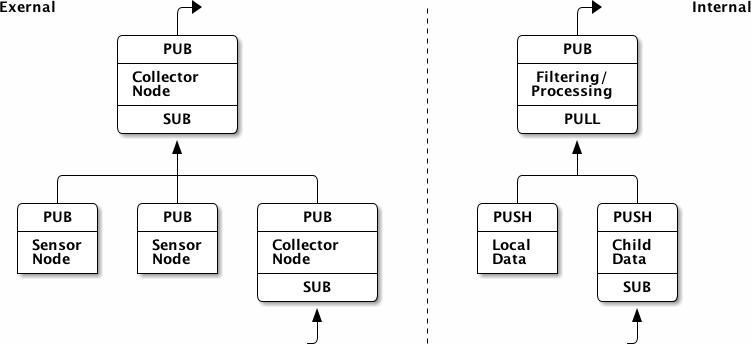
\includegraphics[scale=0.66]{data.png}
    \caption{Data Flow Diagram}
    \label{fig:proto_data_image}
\end{figure}

The \dcamp data flow protocol is very simple, comprised of a single data message type and a heartbeat message type. The
data flows from one node to another via PUB/SUB sockets. Internally, data flows from the upstream data producers,
through a filtering/processing unit, and out to downstream data consumers.

When data rate is slower than a predefined threshold, heartbeats are sent instead to keep inter-node connections alive.

\begin{figure}[ht]
\vspace{+10pt}
\begin{verbatim}
data-flow = *( METRIC / HUGZ )
\end{verbatim}
\vspace{-5pt}
\caption[Data Flow Specification]
	{Data Flow Specification: All messages are sent from child (Metric or Collector) to parent (Collector or Root).}
\label{fig:proto_data_spec}
\end{figure}

\subsubsection{Metric Types}

A metric message must contain: source (node or aggregation), type (e.g. basic, sum, etc.), time (or range), value(s)
(possibly numerator and denominator). Should these types be raw until collected by the root node?

\begin{itemize}
\item basic -- v1 = value at t1, v2 = empty, t2 = empty
\item sum -- v1 = sum at t1, v2 = empty, t2 = empty
\item average -- v1 = sum between t1 and t2, v2 = count
\item percent -- v1 = numerator at t1, v2 = denominator at t1, t2 = empty
\item rate -- v1 = value at t1, v2 = value at t2
\end{itemize}

NOTE ABOUT ACCUMULATION (DOESN'T WORK)

\begin{itemize}
\item filtering can be done two ways: accumulatively and discretely.
\item accumulative means we send only one final value for each time range (e.g. collect every second but report every
      minute, so 60 samples are combined into a single value and sent)
\item discrete means we send each constituent value for each time range, but they are "held" until the time limit is
      reached
\item also, how does this interact with value-based limits? these are always discrete?
\item ACTUALLY: accumulation is not valuable for monotonically increasing values--it is the same as just sampling at the
      slower frequency. accumulation is only valuable for non-monotonically increasing values. but in that case, one
      should find the raw, monotonically increasing values from which it is calculated.
\end{itemize}

\subsubsection{Metric Extensions}

\textbf{VARIABLE LENGTH DATA}
Does \dcamp need to support arbitrary data lengths?

\textbf{NESTED METRICS}
It could be possible for data messages to contain nested data messages, e.g. average/sum of rates.

\textbf{GROUPINGS}
\dcamp may need a more compact data message format for combining multiple metrics into a single message, e.g. for
aggregation purposes or representing entire branches in the topology.
group by source/type/time?
group start/end frames?

\textbf{HISTOGRAMS}
\dcamp should provide a metric histogram ability. Perhaps this should done at each node or only at the root.

\textbf{METRIC REQUESTS}
The admin can use \dcamp to request metrics on a one-time basis, for example, to enumerate the available disks on each
node. The key here is a metric collection is not based on configuration file but rather on real-time input from the
end-user.

Perhaps there should be some special, e.g. "once", metric collection specifications so config data can be sent up to the
root only at node start.

\subsubsection{Message Definitions}

\textbf{METRIC} \\
message containing performance metric data; value v2 will be empty for basic and sum metric types; time t2 will NOT be
empty for average and rate metric types; in case of HUGZ message type, no other property strings are used and frames 3 -
5 are all empty. The config property is only present for internal messages (sent from Sensor to Filter) and represents
the metric configuration's unique name.

\begin{verbatim}
Frame 0: data source (leaf or collector node endpoint), as 0MQ string
Frame 1: properties, JSON-encoded, as 0MQ string
Frame 2: time t1 in ms epoch utc, 8 bytes in network order
Frame 3: value v1, 8 bytes in network order
Frame 4: time t2 in ms epoch utc, 8 bytes in network order; not empty for average and rate
Frame 5: value v2, 8 bytes in network order; empty for basic and sum

properties = *( type / detail / config )
type       = "type=" ( "HUGZ" / "basic" / "sum" / "average" / "percent" / "rate" )
detail     = "detail=" <string>
config     = "config-name=" <string>
\end{verbatim}
